
\documentclass{standalone}

\usepackage{tikz}

\begin{document}

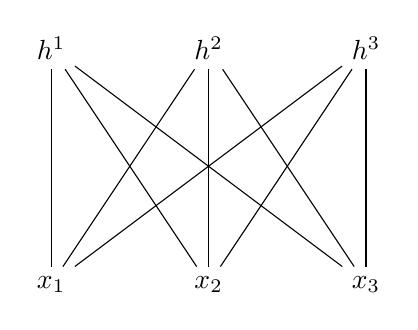
\begin{tikzpicture}
	
\node (h1) at (2,3)		{ $  h^1  $  };
\node (h2) at (4,3)		{ $  h^2  $  };
\node (h3) at (6,3)		{ $  h^3  $  };

\node (x1) at (2,0)		{ $  x_1  $  };
\node (x2) at (4,0)		{ $  x_2  $  };
\node (x3) at (6,0)		{ $  x_3  $  };

\path (h1) edge [draw] (x1);
\path (h1) edge [draw] (x2);
\path (h1) edge [draw] (x3);

\path (h2) edge [draw] (x1);
\path (h2) edge [draw] (x2);
\path (h2) edge [draw] (x3);

\path (h3) edge [draw] (x1);
\path (h3) edge [draw] (x2);
\path (h3) edge [draw] (x3);



\end{tikzpicture}

\end{document}
